\chapter{Removed} % Main appendix title

\label{Removed}

\section{Goodness of steer results}

% REMOVED because plots were generated with an incorrect understanding of 
% what tcpflow logs actually contained.

To compare models, the $G_s$ (Eq. \ref{eq:goodness_of_steer}) was used. Figure  \ref{fig:genTrackOneLap_20201120171015_sanity_gos} contains (discuss):
\begin{itemize}
    \item[--] The PID effect
    \item[--] 
\end{itemize}
The
A second data output was created for the Generated Track circuit. (TODO, create another dataset and plot to compare PID to and manual steering angles).
A video was then created to observe steering angles while recording another dataset on the same lap \href{https://youtu.be/zAmr7a1ImEY}{https://youtu.be/zAmr7a1ImEY}. The video shows steering corrections
% nb recorded at

\begin{figure}[ht]
 \centering 
 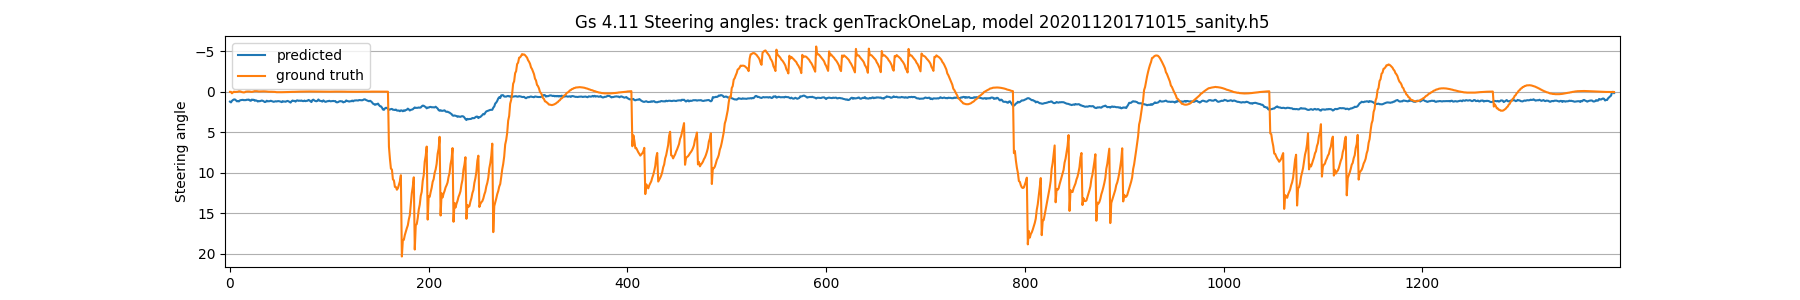
\includegraphics[width=\textwidth]{Figures/sa_genTrackOneLap_20201120171015_sanity.h5.png}
 \caption{Plot containing ground truth steering values recorded in dataset genTrackOneLap .json files and values predicted by model 20201120171015\_ sanity.h5}
 \label{fig:genTrackOneLap_20201120171015_sanity_gos} 
\end{figure}

To confirm the observed acute steering angle variations, a second lap was recorded, producing the same plot
 \label{fig:a_genTrackOneLap_2_20201120171015_sanity} 

\begin{figure}[ht]
 \centering 
 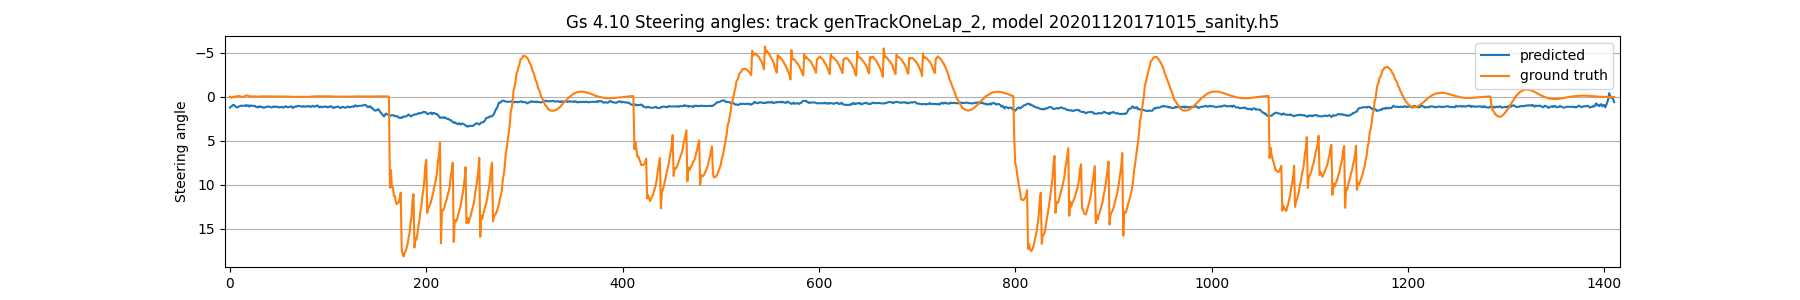
\includegraphics[width=\textwidth]{Figures/sa_genTrackOneLap_2_20201120171015_sanity.h5.png}
 \caption{Plot containing ground truth steering values recorded in dataset genTrackOneLap\_ 2 .json files and values predicted by model 20201120171015\_ sanity.h5, confirming the acute steering angles observed in previous dataset}
 \label{fig:a_genTrackOneLap_2_20201120171015_sanity} 
\end{figure}

The values of Prop and Diff (Proportional and Derivative components of PID steering) were changed while observing steering 
% PID 25, Diff 8, max speed 1.6

This had a smoothing effect to the steering, though the $Gs$ increased:
 \ref{fig:genTrackOneLap_3_20201120171015_sanity_gos} 
 
\begin{figure}[ht]
 \centering 
 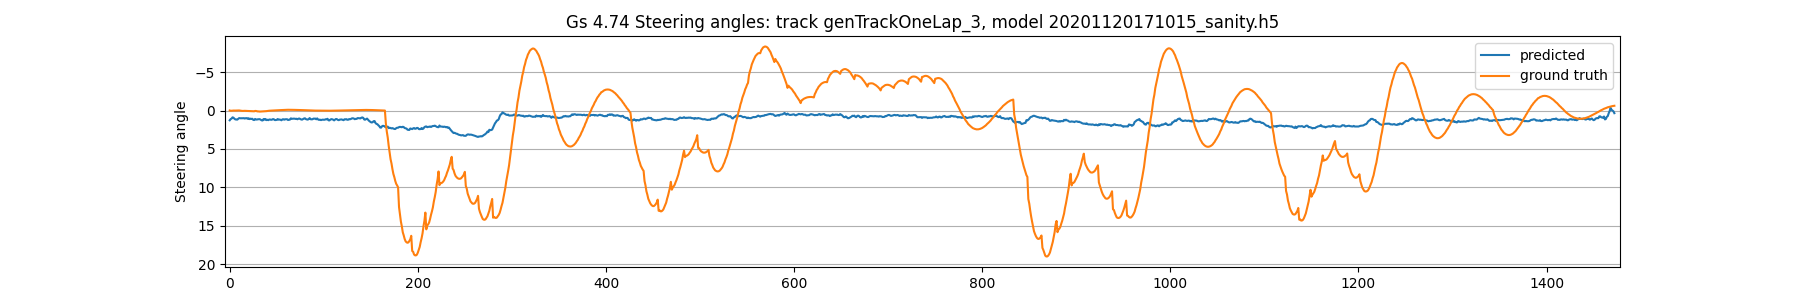
\includegraphics[width=\textwidth]{Figures/sa_genTrackOneLap_3_20201120171015_sanity.h5.png}
 \caption{Plot containing ground truth steering values recorded in dataset genTrackOneLap\_ 3 .json files and values predicted by model 20201120171015\_ sanity.h5, showing the smoothing effect of changing Prop and Diff variables for data capture in Auto w Drive mode}
 \label{fig:genTrackOneLap_3_20201120171015_sanity_gos} 
\end{figure}